%\documentclass[portrait,final,a0paper]{baposter}
\documentclass[a4shrink,portrait,final]{baposter}
% Usa a4shrink for an a4 sized paper.

\tracingstats=2

\usepackage{calc}
\usepackage{graphicx}
\usepackage{amsmath}
\usepackage{amssymb}
\usepackage{relsize}
\usepackage{multirow}
\usepackage{bm}

\usepackage{graphicx}
\usepackage{multicol}

\usepackage{pgfbaselayers}
\pgfdeclarelayer{background}
\pgfdeclarelayer{foreground}
\pgfsetlayers{background,main,foreground}

\usepackage{times}
\usepackage{helvet}
%\usepackage{bookman}
\usepackage{palatino}

\newcommand{\captionfont}{\footnotesize}

\selectcolormodel{cmyk}

\graphicspath{{images/}}


%%%%%%%%%%%%%%%%%%%%%%%%%%%%%%%%%%%%%%%%%%%%%%%%%%%%%%%%%%%%%%%%%%%%%%%%%%%%%%%%
%%%% Some math symbols used in the text
%%%%%%%%%%%%%%%%%%%%%%%%%%%%%%%%%%%%%%%%%%%%%%%%%%%%%%%%%%%%%%%%%%%%%%%%%%%%%%%%
% Format 
\newcommand{\Matrix}[1]{\begin{bmatrix} #1 \end{bmatrix}}
\newcommand{\Vector}[1]{\Matrix{#1}}
\newcommand*{\SET}[1]  {\ensuremath{\mathcal{#1}}}
\newcommand*{\MAT}[1]  {\ensuremath{\mathbf{#1}}}
\newcommand*{\VEC}[1]  {\ensuremath{\bm{#1}}}
\newcommand*{\CONST}[1]{\ensuremath{\mathit{#1}}}
\newcommand*{\norm}[1]{\mathopen\| #1 \mathclose\|}% use instead of $\|x\|$
\newcommand*{\abs}[1]{\mathopen| #1 \mathclose|}% use instead of $\|x\|$
\newcommand*{\absLR}[1]{\left| #1 \right|}% use instead of $\|x\|$

\def\norm#1{\mathopen\| #1 \mathclose\|}% use instead of $\|x\|$
\newcommand{\normLR}[1]{\left\| #1 \right\|}% use instead of $\|x\|$

%%%%%%%%%%%%%%%%%%%%%%%%%%%%%%%%%%%%%%%%%%%%%%%%%%%%%%%%%%%%%%%%%%%%%%%%%%%%%%%%
% Multicol Settings
%%%%%%%%%%%%%%%%%%%%%%%%%%%%%%%%%%%%%%%%%%%%%%%%%%%%%%%%%%%%%%%%%%%%%%%%%%%%%%%%
\setlength{\columnsep}{0.7em}
\setlength{\columnseprule}{0mm}


%%%%%%%%%%%%%%%%%%%%%%%%%%%%%%%%%%%%%%%%%%%%%%%%%%%%%%%%%%%%%%%%%%%%%%%%%%%%%%%%
% Save space in lists. Use this after the opening of the list
%%%%%%%%%%%%%%%%%%%%%%%%%%%%%%%%%%%%%%%%%%%%%%%%%%%%%%%%%%%%%%%%%%%%%%%%%%%%%%%%
\newcommand{\compresslist}{%
\setlength{\itemsep}{1pt}%
\setlength{\parskip}{0pt}%
\setlength{\parsep}{0pt}%
}


%%%%%%%%%%%%%%%%%%%%%%%%%%%%%%%%%%%%%%%%%%%%%%%%%%%%%%%%%%%%%%%%%%%%%%%%%%%%%%
%%% Begin of Document
%%%%%%%%%%%%%%%%%%%%%%%%%%%%%%%%%%%%%%%%%%%%%%%%%%%%%%%%%%%%%%%%%%%%%%%%%%%%%%

\begin{document}

%%%%%%%%%%%%%%%%%%%%%%%%%%%%%%%%%%%%%%%%%%%%%%%%%%%%%%%%%%%%%%%%%%%%%%%%%%%%%%
%%% Here starts the poster
%%%---------------------------------------------------------------------------
%%% Format it to your taste with the options
%%%%%%%%%%%%%%%%%%%%%%%%%%%%%%%%%%%%%%%%%%%%%%%%%%%%%%%%%%%%%%%%%%%%%%%%%%%%%%
% Define some colors
\definecolor{silver}{cmyk}{0,0,0,0.3}
%\definecolor{coral}{cmyk}{0,0.5,0.69,0.0}
\definecolor{coral}{cmyk}{0,0.58,0.69,0.0}
\definecolor{lightcoral}{cmyk}{0,0.48,0.59,0.0}
\definecolor{black}{cmyk}{0,0,0.0,1.0}
\definecolor{darkYellow}{cmyk}{0,0,1.0,0.5}
\definecolor{darkSilver}{cmyk}{0,0,0,0.1}
\definecolor{darksalmon}{cmyk}{0,0.36,0.48,0.09}
\definecolor{salmon5}{cmyk}{0,0.41,0.41,0.56}

\definecolor{lightercoral}{cmyk}{0,0.25,0.25,0}
%\definecolor{lightercoral}{cmyk}{0,0.40,0.47,0.08}
\definecolor{apricot}{cmyk}{0.0,0.36,0.57,0.02}
\definecolor{lightestapricot}{cmyk}{0,0,0.05,0.0}

%%
\typeout{Poster Starts}
\background{
  \begin{tikzpicture}[remember picture,overlay]%
    %\draw (current page.north west)+(-2em,2em) node[anchor=north west] {\includegraphics[height=1.1\textheight]{silhouettes_background}};

  \end{tikzpicture}%
}

\newlength{\leftimgwidth}
\begin{poster}%
  % Poster Options
  {
  % Show grid to help with alignment
  grid=no,
  % Column spacing
  colspacing=1em,
  % Color style
%  bgColorOne=white,
%  bgColorOne=darksalmon,
  bgColorOne=white,
  borderColor=coral,
  %headerColorOne=salmon5,
  headerColorOne=white,
  %headerColorTwo=lightercoral,
  %headerFontColor=lightcoral,
  %boxColorOne=lightercoral,
  boxColorOne=white,
  boxColorTwo=lightercoral,
  % Format of textbox
  textborder=roundedleft,
%  textborder=rectangle,
  % Format of text header
  eyecatcher=yes,
  headerborder=open,
  headerheight=0.08\textheight,
  headershape=roundedright,
  headershade=plain,
  headerfont=\Large\textsf, %Sans Serif
  boxshade=plain,
%  background=shade-tb,
  background=plain,
  linewidth=1pt
  }
  % Eye Catcher
  {
\includegraphics[height=7.0em]{ntua_logo.pdf}} % No eye catcher for this poster. (eyecatcher=no above). If an eye catcher is present, the title is centered between eye-catcher and logo.
  % Title
  {\sf %Sans Serif
  %\bf% Serif
  %\vspace{1em}
  V4VSockets: low overhead intra-node communication in Xen}
  % Authors
  {\sf %Sans Serif
  % Serif
  A. Nanos, S. Gerangelos, I. Alifieraki and N. Koziris\\
  \{ananos,sgerag,ialif,nkoziris\}@cslab.ece.ntua.gr
  }
  % University logo
  {% The makebox allows the title to flow into the logo, this is a hack because of the L shaped logo.
    \makebox[8em][r]{%
      \begin{minipage}{16em}
        \hfill
        
\includegraphics[height=4em]{cslab_logo.pdf}
        %
\includegraphics[height=7.0em]{ntua_logo.pdf}
      \end{minipage}
    }
  }

  \tikzstyle{light shaded}=[top color=baposterBGtwo!30!white,bottom color=baposterBGone!30!white,shading=axis,shading angle=30]

  % Width of left inset image
     \setlength{\leftimgwidth}{0.78em+8.0em}

%%%%%%%%%%%%%%%%%%%%%%%%%%%%%%%%%%%%%%%%%%%%%%%%%%%%%%%%%%%%%%%%%%%%%%%%%%%%%%
%%% Now define the boxes that make up the poster
%%%---------------------------------------------------------------------------
%%% Each box has a name and can be placed absolutely or relatively.
%%% The only inconvenience is that you can only specify a relative position 
%%% towards an already declared box. So if you have a box attached to the 
%%% bottom, one to the top and a third one which should be in between, you 
%%% have to specify the top and bottom boxes before you specify the middle 
%%% box.
%%%%%%%%%%%%%%%%%%%%%%%%%%%%%%%%%%%%%%%%%%%%%%%%%%%%%%%%%%%%%%%%%%%%%%%%%%%%%%
    %
    % A coloured circle useful as a bullet with an adjustably strong filling
    \newcommand{\colouredcircle}[1]{%
      \tikz{\useasboundingbox (-0.2em,-0.32em) rectangle(0.2em,0.32em); \draw[draw=black,fill=baposterBGone!80!black!#1!white,line width=0.03em] (0,0) circle(0.18em);}}

%%%%%%%%%%%%%%%%%%%%%%%%%%%%%%%%%%%%%%%%%%%%%%%%%%%%%%%%%%%%%%%%%%%%%%%%%%%%%%
  \headerbox{Motivation}{name=motivation,column=0,row=0, span=3}{
%%%%%%%%%%%%%%%%%%%%%%%%%%%%%%%%%%%%%%%%%%%%%%%%%%%%%%%%%%%%%%%%%%%%%%%%%%%%%%

In the HPC context, applications often scale to a large number of nodes,
leading to the need for a high-performance interconnect to provide low-latency
and high-bandwidth communication. 

In the cloud context, distributed applications are executed in a set of Virtual
Machines (VMs) that are placed in physical nodes across the cloud data center.
These VMs suffer \emph{communication overheads} and are \emph{unaware of their
physical placement} -- this presents a problem, because application instances
running on the same physical node but on different VMs are not able to
\emph{exploit locality}. 

Additionally, the advent of Software Defined Networks and
Network Function Virtualization (commonly referred to as SDN/NFV) has given
rise to examine approaches where lightweight VMs exchange data with co-located
peers to perform \emph{data-intensive network processing operations}.

\vspace{1em}
}

%%%%%%%%%%%%%%%%%%%%%%%%%%%%%%%%%%%%%%%%%%%%%%%%%%%%%%%%%%%%%%%%%%%%%%%%%%%%%%
  \headerbox{Contribution}{name=contribution,column=0, below=motivation}{
%%%%%%%%%%%%%%%%%%%%%%%%%%%%%%%%%%%%%%%%%%%%%%%%%%%%%%%%%%%%%%%%%%%%%%%%%%%%%%
$\Rightarrow$ We introduce V4VSockets, an efficient, socket-compliant,
high--performance intra-node communication framework.

$\Rightarrow$ We evaluate V4VSockets using generic micro-benchmarks and compare
it to conventional communication paths. We find that V4VSockets outperforms the
generic method of intra-node communication and scales efficiently with a large
number of VMs both in terms of throughput as well as latency.

$\Rightarrow$ We present a real-life use case: we deploy an HPC application
stencil over rCUDA, a remote GPU execution stack over V4VSockets.

\vspace{1em}
}

%%%%%%%%%%%%%%%%%%%%%%%%%%%%%%%%%%%%%%%%%%%%%%%%%%%%%%%%%%%%%%%%%%%%%%%%%%%%%%%
%  \headerbox{I/O Path}{name=network path,row=0,column=1,span=2}{
%%%%%%%%%%%%%%%%%%%%%%%%%%%%%%%%%%%%%%%%%%%%%%%%%%%%%%%%%%%%%%%%%%%%%%%%%%%%%%%
%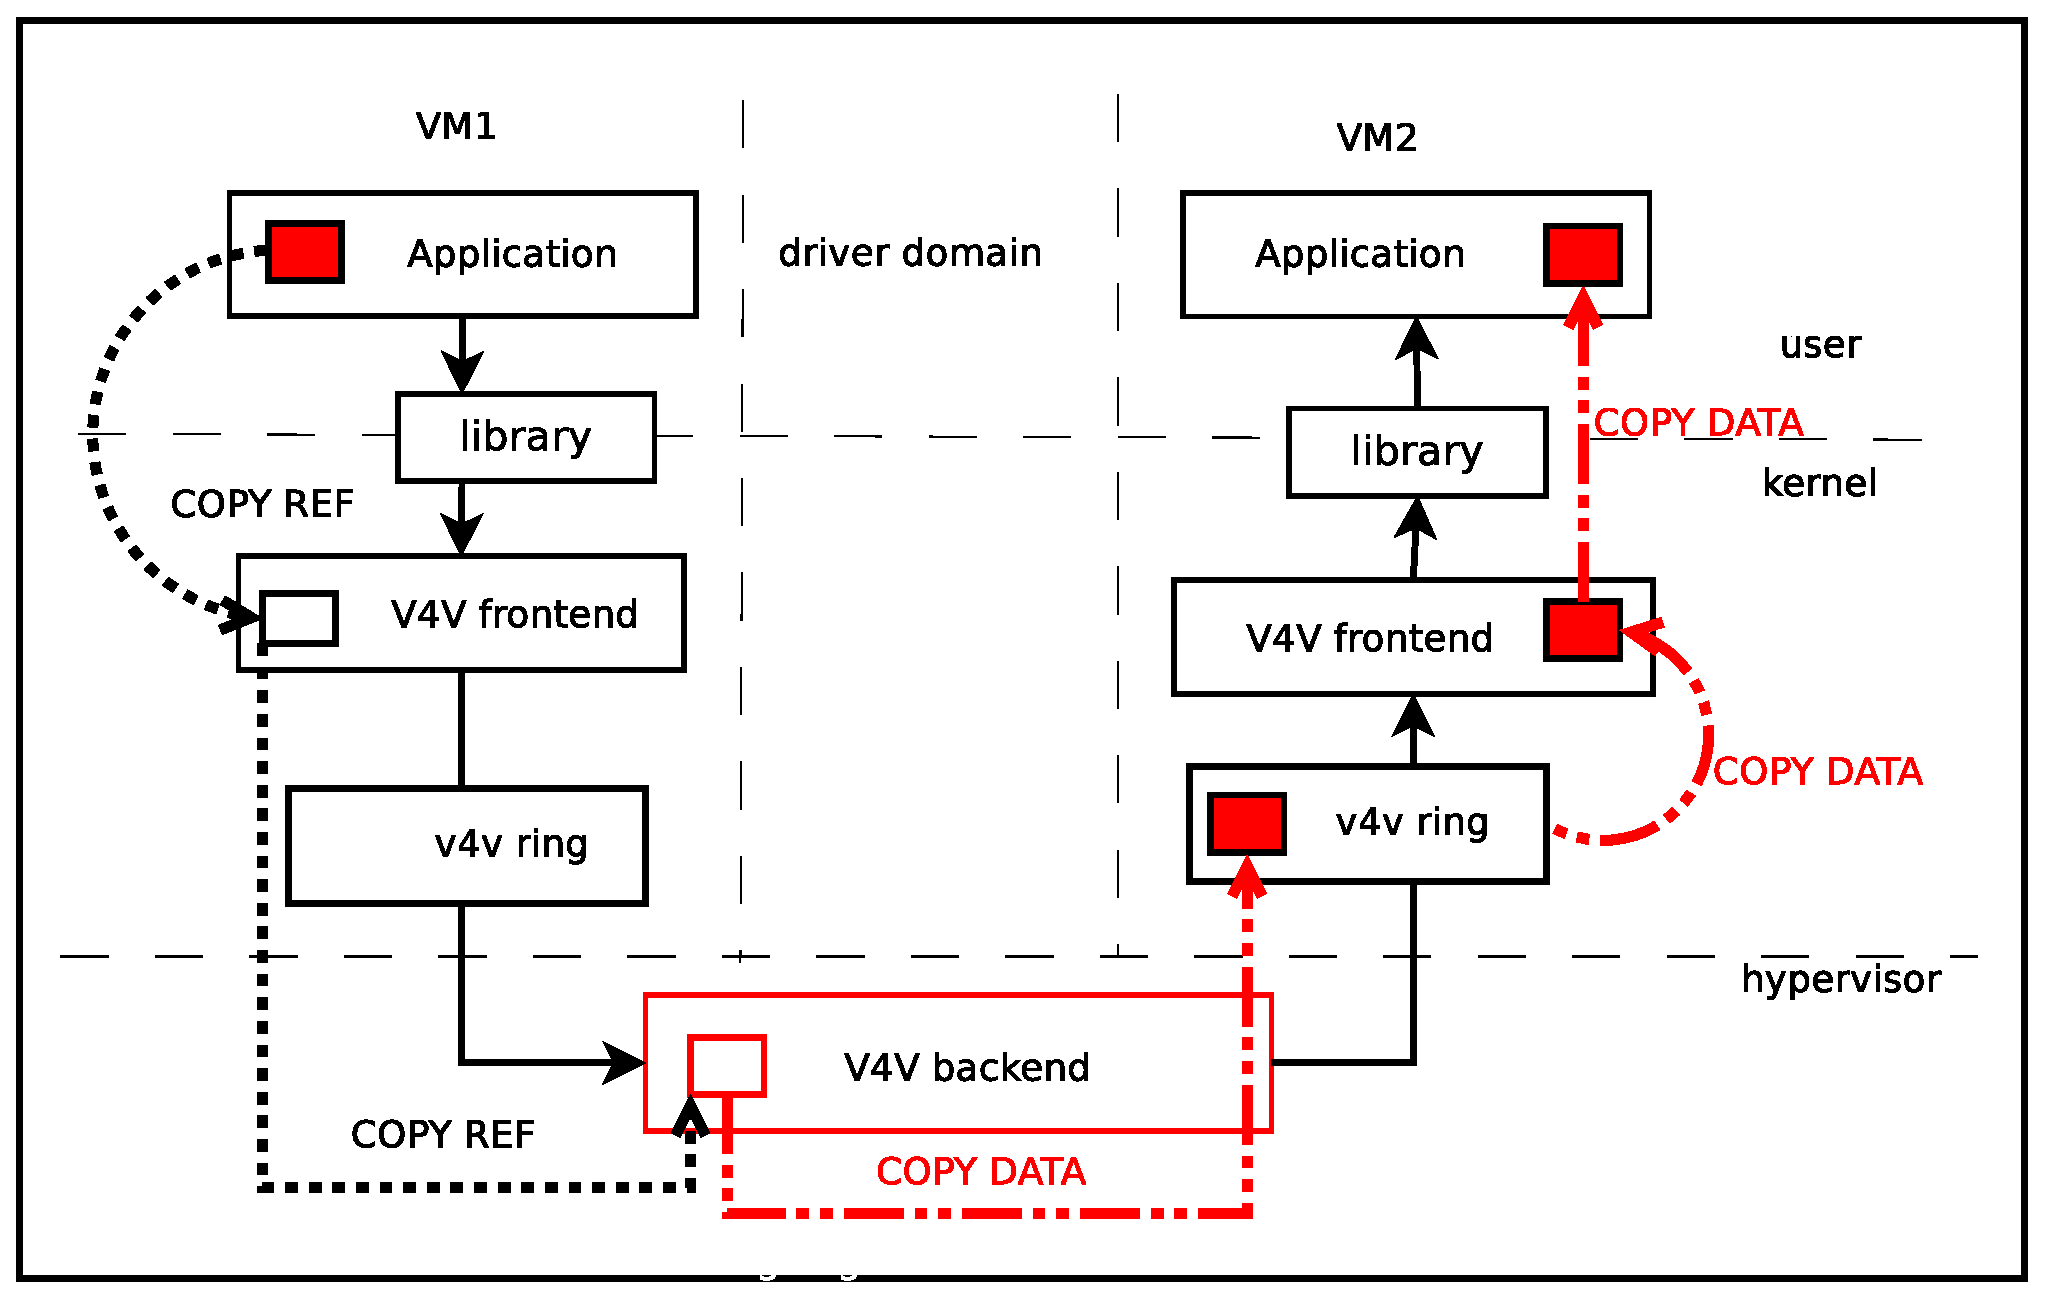
\includegraphics[width=.5\linewidth]{figures/v4vsockets.eps}
%%\includegraphics[width=.5\linewidth]{}
%  }
%%%%%%%%%%%%%%%%%%%%%%%%%%%%%%%%%%%%%%%%%%%%%%%%%%%%%%%%%%%%%%%%%%%%%%%%%%%%%%%%
%% \headerbox{Acknowledgements}{name=acknowledgements,column=0,above=bottom}{
%%%%%%%%%%%%%%%%%%%%%%%%%%%%%%%%%%%%%%%%%%%%%%%%%%%%%%%%%%%%%%%%%%%%%%%%%%%%%%%%
%%  \small
%%%  \hspace{1em}
%%   The authors would like to thank Nikos Nikoleris, Elisavet Kozyri and Stratos Psomadakis for their usefull contributions to this work.
%%\vspace{0.5em}
%%  }
%
%%%%%%%%%%%%%%%%%%%%%%%%%%%%%%%%%%%%%%%%%%%%%%%%%%%%%%%%%%%%%%%%%%%%%%%%%%%%%%%
%  \headerbox{Preliminary results on HPC cluster interconnects}{name=results,column=1,span=2,below=network path,above=bottom}{%,below=questions}{
%%%%%%%%%%%%%%%%%%%%%%%%%%%%%%%%%%%%%%%%%%%%%%%%%%%%%%%%%%%%%%%%%%%%%%%%%%%%%%%
%%\setlength{\columnseprule}{1pt}
%\setlength{\columnsep}{13pt}
%      \begin{multicols}{2}
%We run the pktgen utility of the Linux kernel. The figure on the right plots
%the maximum achievable socket buffer production rate when ran in vanilla Linux,
%inside the Privileged Guest and in the VM. In the default configuration, Xen's
%virtual ethernet device does not feature specific optimizations and as a
%result, its performance is limited to 416MiB/sec.
%
% \hspace{0.5em}\scalebox{.890}{
%       \includegraphics[width=\linewidth]{baseline_throughput}}
%	\end{multicols}
%
%\vspace{-1em}
%      \mbox{\hspace{0.15\linewidth}\rule{0.7\linewidth}{.8pt}\hspace{0.15\linewidth}}
%
%	\begin{multicols}{2}
%	\begin{center}
%      \begin{tabular}{cc}
%       \hspace{-0.5em}\scalebox{.800}{%\scalebox{0.875}{
%	\includegraphics[width=\linewidth]{bandwidth}}
%      \end{tabular}
%	\end{center}
%	\begin{center}
%        \hspace{0.5em}\scalebox{.800}{\includegraphics[width=\linewidth]{latency}}
%	\end{center}
%	\end{multicols}
%
%	\begin{multicols}{2}
%We use a custom synthetic microbenchmark to evaluate our approach over
%our interconnect sending unidirectional RDMA write requests. To obtain
%a baseline measurement, we implement our microbenchmark using TCP
%sockets. The figure on the left plots the aggregate throughput of the
%system.
%Specifically, we deployed our microbenchmark on top of TCP sockets (filled
%circles) and our framework (filled squares). An RDMA message over TCP sockets
%takes 77$\mu$sec to cross the network whereas over our framework takes
%28$\mu$sec (Figure on the right).
%	\end{multicols}
%\vspace{-1em}
%      \mbox{\hspace{0.15\linewidth}\rule{0.7\linewidth}{.8pt}\hspace{0.15\linewidth}}
%      \begin{multicols}{2}
%	\begin{center}
%	\hspace{-0.5em}\scalebox{.88}{\includegraphics[width=\linewidth]{dom0_cpu_util}} 
%	\end{center}
%	\begin{center}
%	\hspace{-0.5em}\scalebox{1}{\includegraphics[width=\linewidth]{domU_cpu_util}}
%	\end{center}
%
%      \end{multicols}
%
%      \begin{multicols}{2}
%We measure the total CPU time when two VMs perform RDMA writes of
%varying message sizes over the network (TCP and ZERO\_COPY approach). To investigate the sources of CPU time consumption, we perform
%a detailed breakdown of the subsystems used in the RDMA operations for
%TCP and our framework. The figures above plot the CPU time breakdown for the
%Privileged Guest (left) and the VM (right). 
%	\end{multicols}
%
%
%  \vspace{0.5em}
%  }

%%%%%%%%%%%%%%%%%%%%%%%%%%%%%%%%%%%%%%%%%%%%%%%%%%%%%%%%%%%%%%%%%%%%%%%%%%%%%%%
%  \headerbox{Open Challenges}{name=questions,column=0,span=1,below=contribution}{
%%%%%%%%%%%%%%%%%%%%%%%%%%%%%%%%%%%%%%%%%%%%%%%%%%%%%%%%%%%%%%%%%%%%%%%%%%%%%%%
%    
%\textit{Higher-level parallel frameworks}: Our protocol implements simple RDMA semantics
%(READ, WRITE). We are in the process of extending its capabilities to support
%higher-level frameworks for application parallelism such as MPI or MapReduce.
%
%\textit{Performance}: Efficient I/O device sharing and support in Virtualized
%environments does not appear to be sufficiently mature. Even in full
%virtualization setups, many I/O devices have to be exported as emulated devices
%to VMs. %In this work, we observe suboptimal performance when transferring data
%%from VMs to network using common generic approaches (such as TCP/IP over 10GbE
%%adapters), while at the same time CPU cores were busy multiplexing accesses to
%%the hardware. 
%%In order to be able to deploy HPC applications in VM
%%environments, we have to take into account overheads imposed by Virtualization
%%layers and eliminate them. 
%
%\textit{Hardware Offloading}: Our prototype implementation consists of a frontend and a
%backend in the Xen virtualization platform. We show that while in the frontend
%part (VM) CPU time is negligible and agnostic to varying message sizes, there
%is still some CPU time spent in the Driver domain that can potentially reduce
%the performance of the entire system. This issue could be resolved by
%offloading this thin protocol layer to a hardware device, capable of performing
%DMA transfers and simple protocol processing. 
%%In addition to that, using SR-IOV
%%techniques with this custom device can lead to a VM-capable, high-performance
%%interconnection architecture over 10G Ethernet, comparable to VIA
%%Myrinet/Infiniband for virtualized environments. %To this end, we are in the
%%process of evaluating our approach in a custom, programmable controller
%%equipped with a 10GbE interface. We aspire to alleviate all CPU overheads
%%associated with protocol processing and propose optimizations that can achieve
%%near-native performance.
%
%\textit{Decoupling HPC from the Privileged Guest}: While a hardware approach, as
%mentioned above, could resolve CPU time issues, 
%we would like to examine the
%possibility of decoupling all HPC network-related issues to a different domain.
%This way, overheads associated with world switches and interrupt handling can
%be alleviated. We plan on evaluating this idea based on Xen stub domains, using
%modular networking components that can be easily implemented and optimized.
%   
%  }

\end{poster}

\end{document}
